% -----------------------------------------------
% Template for ISMIR 2014
% (based on earlier ISMIR templates)
% -----------------------------------------------

\documentclass{article}
\usepackage{ismir2014,amsmath,cite}
\usepackage{graphicx}
\usepackage{multirow}

% Title.
% ------
\title{DRUM TRANSCRIPTION IN POLYPHONIC MUSIC USING SEMI-SUPERVISED NON-NEGATIVE MATRIX FACTORIZATION}

% Single address
% To use with only one author or several with the same address
% ---------------
%\oneauthor
% {Names should be omitted for double-blind reviewing}
% {Affiliations should be omitted for double-blind reviewing}

% Two addresses
% --------------
%\twoauthors
%  {First author} {School \\ Department}
%  {Second author} {Company \\ Address}

% Three addresses
% --------------
\threeauthors
  {First author} {Affiliation1 \\ {\tt author1@ismir.edu}}
  {Second author} {\bf Retain these fake authors in\\\bf submission to preserve the formatting}
  {Third author} {Affiliation3 \\ {\tt author3@ismir.edu}}

% Four addresses
% --------------
%\fourauthors
%  {First author} {Affiliation1 \\ {\tt author1@ismir.edu}}
%  {Second author}{Affiliation2 \\ {\tt author2@ismir.edu}}
%  {Third author} {Affiliation3 \\ {\tt author3@ismir.edu}}
%  {Fourth author} {Affiliation4 \\ {\tt author4@ismir.edu}}

\begin{document}
%
\maketitle
%
\begin{abstract}
In this paper, a drum transcription algorithm using semi-supervised non-negative matrix factorization has been presented. This method allows users to separate percussive activities from harmonic activities with pre-trained drum templates, and detect drum events from the extracted percussive activity matrix. A polyphonic subset from ENST drum dataset has been used for training and testing of the algorithm. The system has been tested using different rank settings, and a cross-performer validation process has been performed to evaluate the reliability of the system.  The results show that the system can achieve 61 to 77\% recognition rate on multiple drums in polyphonic music. In the future, more efforts will be put on differentiating different playing styles and more drum parts, leading toward a complete drum transcription system.

\end{abstract}
%

\section{Introduction}\label{sec:introduction}
Transcribing music content into sheet music or any form of score is an essential skill to musicians for analysis and composition purposes. However, It is often considered a time-consuming and non-trivial task, for it requires repetitive listening and integral knowledge of music and instruments. With the advance of computing power and various machine learning techniques, a system that has the abilities to automatically recognize music content has become a plausible idea and interests many researchers in the field of Music Information Retrieval (MIR) [1]. In general, Automatic Music Transcription (AMT) systems could not only serve as a tool to record the music content, identify notes from improvisations, but also lead to the realization of a music intelligence system [2]. To build a complete AMT system, many subtasks and challenges, such as multi-pitch detection, onset detection, instrument recognition, and rhythm extraction, have been attempted [1]. Comparing with pitched instruments, transcribing un-pitched music events such as percussive sounds seem to be less addressed, and a robust algorithm to detect drum sounds in polyphonic music is still an open question in this field.

Drum track, especially in pop music, often plays an important role in determining music structure, style, rhythm and tempo. In many cases, it shares the same importance as the harmonic part in the music. That said, a good drum transcription system could provide essential information of the music content, and could potentially facilitate the realization of many interesting applications. For example, a drum transcription and drum source separation task could mutually benefit from each other and provide the possibility to manipulate drum sounds within an existing drum track [3], [4].  Also, music education could be an application of a drum transcription system, for it could help students identify drum event within a polyphonic music, and provide instructions by analyzing and comparing the differences between the input and reference performances. Furthermore, such system could also be integrated as a part of machine listening, improving the existing systems of robotic musicians[5].

Therefore, this study aims to explore alternative solutions to drum transcription in polyphonic music. The final goal of this paper is to find a potential direction to push the limit of this task, leading toward further musical applications.

\section{Related Works}\label{sec:related works}
The early attempts to transcribe percussive sounds main focused on classifying monophonic signals [6][7]. With standard approaches such as feature extraction and classification, fairly high accuracy were reported in the previous studies. However, in the real use case, a drum transcription system is expected to work in polyphonic signal instead of monophonic. Therefore, solving this problem in the context of polyphonic music had become another criterion, and different methods could be found in previous research [8]–[15].  According to [15], recent studies on the drum transcription in polyphonic music could be categorized into three types: segment and classify, separate and detect, match and adapt.  For the first type of approaches, the common procedure starts by applying onset detection to the audio signal in order to segment the music event. Once the event has been detected, various features from time or spectral domain of the signal will be extracted, and a classifier will be trained to classify the event based on the extracted features. This type of approaches seem to perform well when the data and features are well chosen [13], [15]. However, to get good results, sufficient amount of data, careful preprocessing and training steps are required in this type of systems. Additionally, to handle the situation of simultaneous sounds, more classes need to be trained.

The second type of approaches is based on the assumption that music signal is a superposition of different sound sources. By decomposing the signal and into different source templates and corresponding activities, the music content could be transcribed by detecting onsets of these activities. Different methods such as Independent Subspace Analysis (ISA) [16], Prior Subspace Analysis (PSA) [8], and Non-negative Matrix Factorization (NMF) [14], [17], [18] are the examples in this category. This type of approaches is usually easier to interpret, since most of the decompositions have been done on the spectrogram of the signal. Also, the separate nature allows simultaneous events to be handled easily in this case. However, to be able to transcribe different kinds of music, a large template might be required prior to the decomposition. Moreover, the number of rank during the decomposition process could be difficult to determine in some cases. 

The third type of approaches uses pre-trained templates to detect drum events [19][20]. An iterative process has been taken to search for the closest matches to these templates and adapt them. The proposed system has been evaluated and performed well in MIREX 2005 drum detection competition. However, to coverage a wider range of sounds, multiple seed templates need to be prepared prior to the process.

In this paper, an approach that falls into the second category has been presented. Based on the popular NMF based  
\section{Method}\label{sec:method}
about 1 page

\subsection{Algorithm Description}\label{subsec:algorithm description}

This part I will first mention the co-factorization paper, and then introduce my modification of the algorithm, the cost function and the updating methods...

\subsection{Processing Steps}\label{subsec:processing steps}

Here I will put my system flowchart, and explain my processing procedure step by step. 




%============= System + high pass figure here
\begin{figure}
 \centerline{\framebox{
 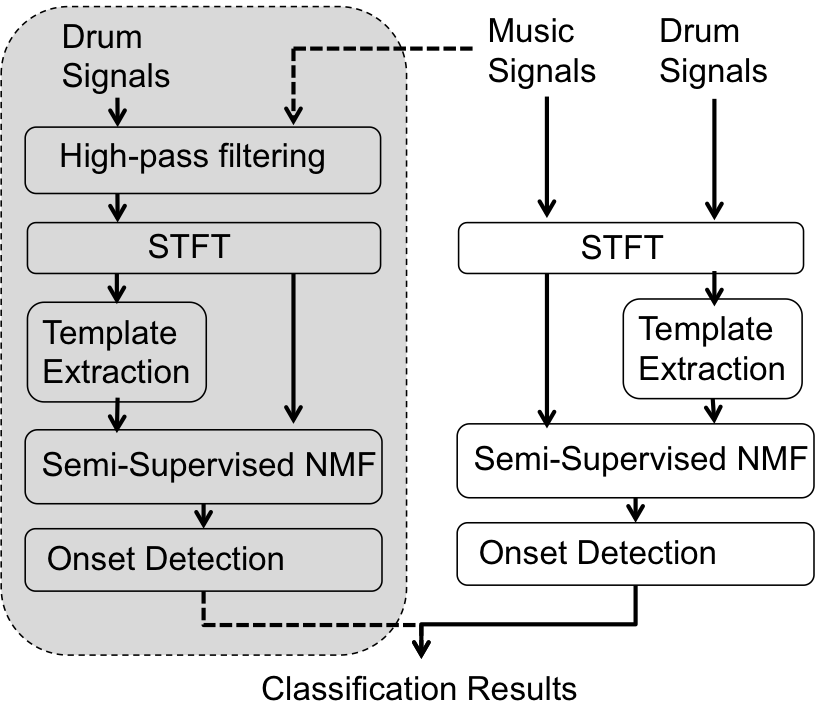
\includegraphics[width=\columnwidth]{flowchart.png}}}
 \caption{Flowchart of the drum transcription system.}
 \label{fig:flowchart}
\end{figure}





\subsubsection{Template Extraction}\label{subsubsec:template extraction}
1)extract templates



\subsubsection{Activity Detection}\label{subsubsec:activity detection}
2)thresholding on activity matrix


\section{Evaluation}\label{sec:Evaluation}

about 2 pages

\subsection{Dataset Description}\label{subsec:dataset description}

1)dataset description

In this project, all of the experiments have been conducted on the “minus one” subset from the ENST public drum dataset [22].  This dataset consist of recordings from three different drummers performing on their own drum kits. The recording contains single hits on different drums, short phrases of drum beats, drum solos, and short play through with the accompaniments. The minus one public subset has 64 tracks of polyphonic music; each track has a length of approximately 70 seconds. The music style varies from each other. Particularly, this subset contains many drum playing techniques such as ghost notes, flam, and drag…etc, which could be considered difficult for many of the existing drum transcription algorithms. The accompaniments are mixed with the “wet mix” in the dataset without any modification of the magnitudes.   

The onset counts of each class within different drummer’s recordings are shown in Table 1. More details on the creation process of this dataset could be found in their corresponding paper. 

%============= Onset event counts in the used tracks
\begin{table}[h]
\begin{center}
\begin{tabular}{|c|c|c|c|c|}
\hline
Drummer\# & 1    & 2    & 3    & Total \\ \hline
HH        & 1942 & 2145 & 1813 & 5900  \\ \hline
BD        & 2140 & 1488 & 1378 & 5006  \\ \hline
SD        & 2165 & 2079 & 1994 & 6238  \\ \hline
Total     & 6247 & 5712 & 5185 & 17144 \\ \hline
\end{tabular}
 \caption{Onset counts in selected dataset.}
 \label{tab:onsetCount}
\end{center}
\end{table}

\subsection{Evaluation Procedure}\label{subsec:evaluation procedure}
To keep classifiers from seeing the data during the training phase, a cross-performer validation process has been performed. As shown in Fig 2, when a drummer’s recordings is selected as the training data, the classifier will be tested using the other drummer’s recordings. The process applies to every drummer’s recordings, and the performance of the training data is the average of the test results from the other two drummers.

The accuracy of the classification has been evaluated by calculating the precision, recall and F-scores. 


one figure here showing the procedure
%============= Cross-performer validation figure
\begin{figure}
 \centerline{\framebox{
 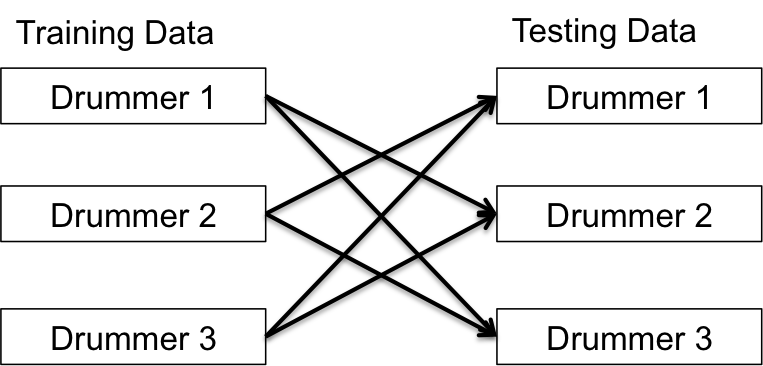
\includegraphics[width=\columnwidth]{cross.png}}}
 \caption{Cross-performer validation process.}
 \label{fig:cross}
\end{figure}






\subsection{Evaluation Results}\label{subsec:evaluation results}

3)basic results + improved results (filtering)


%============= Train on All templates
\begin{table}[h]
\begin{center}
\begin{tabular}{|c|c|c|c|c|}
\hline
\multicolumn{2}{|c|}{}  & Original & HPF+LPF+BPF & HPF only \\ \hline
\multirow{3}{*}{HH} & P & 0.605    & 0.671       & 0.675    \\ \cline{2-5} 
                    & R & 0.713    & 0.737       & 0.736    \\ \cline{2-5} 
                    & F & 0.654    & 0.702       & 0.704    \\ \hline
\multirow{3}{*}{BD} & P & 0.723    & 0.662       & 0.740    \\ \cline{2-5} 
                    & R & 0.837    & 0.855       & 0.839    \\ \cline{2-5} 
                    & F & 0.776    & 0.746       & 0.786    \\ \hline
\multirow{3}{*}{SD} & P & 0.678    & 0.591       & 0.676    \\ \cline{2-5} 
                    & R & 0.566    & 0.583       & 0.569    \\ \cline{2-5} 
                    & F & 0.617    & 0.587       & 0.618    \\ \hline
\end{tabular}
\end{center}
 \caption{Transcription results using all training templates.}
 \label{tab:basic results}
\end{table}

4)system properties (rank change, iteration and convergence, cross training and testing)

%============= Train on Drummer 1 templates
\begin{table}[h]
\begin{center}
\begin{tabular}{|c|c|c|c|c|}
\hline
\multicolumn{2}{|c}{Training} & \multicolumn{3}{|c|}{Drummer 1}   \\ \hline
\multicolumn{2}{|c|}{Testing} & Drummer 1 & Drummer 2 & Drummer 3 \\ \hline
\multirow{3}{*}{HH}    & P    & 0.662     & 0.621     & 0.564     \\ \cline{2-5} 
                       & R    & 0.670     & 0.749     & 0.692     \\ \cline{2-5} 
                       & F    & 0.666     & 0.679     & 0.622     \\ \hline
\multirow{3}{*}{BD}    & P    & 0.620     & 0.781     & 0.850      \\ \cline{2-5} 
                       & R    & 0.393     & 0.914     & 0.900      \\ \cline{2-5} 
                       & F    & 0.481     & 0.842     & 0.874     \\ \hline
\multirow{3}{*}{SD}    & P    & 0.639     & 0.800     & 0.589     \\ \cline{2-5} 
                       & R    & 0.546     & 0.608     & 0.487     \\ \cline{2-5} 
                       & F    & 0.588     & 0.691     & 0.533     \\ \hline
\end{tabular}
 \caption{Transcription results using drummer 1 training templates.}
 \label{tab:trainDr1}
\end{center}
\end{table}

%============= Train on Drummer 2 templates
\begin{table}[h]
\begin{center}
\begin{tabular}{|c|c|c|c|c|}
\hline
\multicolumn{2}{|c}{Training} & \multicolumn{3}{|c|}{Drummer 2}   \\ \hline
\multicolumn{2}{|c|}{Testing} & Drummer 1 & Drummer 2 & Drummer 3 \\ \hline
\multirow{3}{*}{HH}    & P    & 0.661     & 0.600     & 0.541     \\ \cline{2-5} 
                       & R    & 0.667     & 0.787     & 0.699     \\ \cline{2-5} 
                       & F    & 0.664     & 0.681     & 0.610     \\ \hline
\multirow{3}{*}{BD}    & P    & 0.466     & 0.846     & 0.699     \\ \cline{2-5} 
                       & R    & 0.603     & 0.986     & 0.854     \\ \cline{2-5} 
                       & F    & 0.525     & 0.910     & 0.769     \\ \hline
\multirow{3}{*}{SD}    & P    & 0.625     & 0.849     & 0.529     \\ \cline{2-5} 
                       & R    & 0.550     & 0.624     & 0.486     \\ \cline{2-5} 
                       & F    & 0.585     & 0.719     & 0.506     \\ \hline
\end{tabular}
 \caption{Transcription results using drummer 2 training templates.}
 \label{tab:trainDr2}
\end{center}
\end{table}


%============= Train on Drummer 3 templates
\begin{table}[h]
\begin{center}
\begin{tabular}{|c|c|c|c|c|}
\hline
\multicolumn{2}{|c}{Training} & \multicolumn{3}{|c|}{Drummer 3}   \\ \hline
\multicolumn{2}{|c|}{Testing} & Drummer 1 & Drummer 2 & Drummer 3 \\ \hline
\multirow{3}{*}{HH}    & P    & 0.614     & 0.599     & 0.523     \\ \cline{2-5} 
                       & R    & 0.660     & 0.717     & 0.675     \\ \cline{2-5} 
                       & F    & 0.636     & 0.652     & 0.589     \\ \hline
\multirow{3}{*}{BD}    & P    & 0.506     & 0.862     & 0.800     \\ \cline{2-5} 
                       & R    & 0.636     & 0.965     & 0.932     \\ \cline{2-5} 
                       & F    & 0.564     & 0.910     & 0.861     \\ \hline
\multirow{3}{*}{SD}    & P    & 0.477     & 0.615     & 0.564     \\ \cline{2-5} 
                       & R    & 0.580     & 0.598     & 0.534     \\ \cline{2-5} 
                       & F    & 0.523     & 0.607     & 0.548     \\ \hline
\end{tabular}
 \caption{Transcription results using drummer 3 training templates.}
 \label{tab:trainDr3}
\end{center}
\end{table}

%============= Rank Test Figure
\begin{figure}
 \centerline{\framebox{
 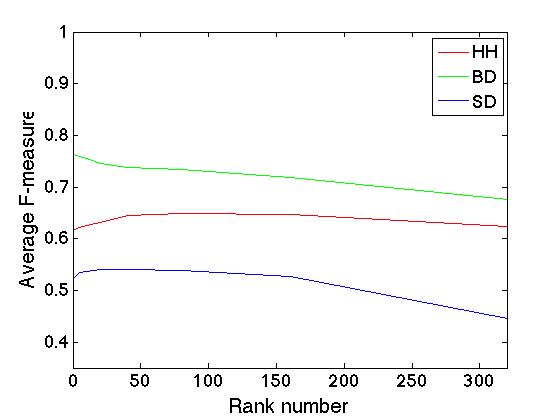
\includegraphics[width=\columnwidth]{rankTest.png}}}
 \caption{Average F-measure versus rank change in harmonic activity matrix.}
 \label{fig:rankTest}
\end{figure}




\subsection{Discussions}\label{subsec:discussions}

5)discussion

although the results seem to be comparable, NMF based method still has some advantages over instance based methods: 1. simultaneous sounds will be detected separately  2. require less labeled data during the training process 3. 




\section{Conclusion}\label{sec:Conclusion}

about 0.5 page


\section{Reference}



%============= This part is for reference only, will be removed once my parts are finished =============
\section{Equations}

Equations should be placed on separated lines and numbered.
The number should be on the right side, in parentheses.

\begin{equation}
E=mc^{2}
\end{equation}

\section{Citations}

All bibliographical references should be listed at the end,
inside a section named ``REFERENCES,'' numbered and in alphabetical order.
Also, all references listed should be cited in the text.
When referring to a document, type the numbering square brackets
\cite{Author:00} or \cite{Author:00,Someone:10,Someone:04}.

\begin{thebibliography}{citations}

\bibitem {Author:00}
E. Author:
``The Title of the Conference Paper,''
{\it Proceedings of the International Symposium
on Music Information Retrieval}, pp.~000--111, 2000.

\bibitem{Someone:10}
A. Someone, B. Someone, and C. Someone:
``The Title of the Journal Paper,''
{\it Journal of New Music Research},
Vol.~A, No.~B, pp.~111--222, 2010.

\bibitem{Someone:04} X. Someone and Y. Someone: {\it Title of the Book},
    Editorial Acme, Porto, 2012.

\end{thebibliography}

%\bibliography{ismir2014template}

\end{document}
